%\documentclass[11pt,emulateapj,apjfonts,epsf]{aastex}
\documentclass[preprint,12pt,longnamesfirst]{aastex}
%\documentclass[manuscript,12pt]{aastex}
%\documentclass[longnamesfirst]{emulateapj}

%\usepackage{emulateapj5}
\usepackage{latexsym}

\shorttitle{}
\shortauthors{}

\newcommand {\kms}{km~s$^{-1}$}
\newcommand{\ud}{\mathrm{d}}

\begin{document}

\title{A Check of the Analytical Model of the Adiabatic
Expansion Cluster Wind}

\author{Wei Sun}
% \affil{Purple Mountain Observatory, CAS}

\begin{abstract}

The power-law approximation is solid, which means there is barely
deceleration toward the expanding wind.

\end{abstract}

% \keywords{Cluster Wind, NGC 3603}

%%%%%%%%%%%%%%%%%%%%%%%%%%%%%%%%%%%%%%%%%%%%%%%%%%%%%%%%%%%%%%%%%%%%%%%%%
\section{Introduction} %Section 1

The check the spectral calculation code of my version, we set up a
benchmark model as presented in Ji et al (2006, \S3.4):
\begin{quote}
\textit{As an illustration, we consider a toy model for an
adiabatically expanding stellar cluster wind with a constant mass
input rate $\dot{M}\sim3\times10^{-5}\,M_\odot$~yr$^{-1}$ and a
constant velocity $v=1000$~km~s$^{-1}$. We assume that the wind is
injected at an initial radius of $r_0=0.3$~pc and is heated up to
a CIE state with an equilibrium temperature $T_0=5\times10^6$~K.
As the wind expands adiabatically,
\textbf{its temperature drops as $T=T_0(r/r_0)^{-4/3}$}.}
\end{quote}

However, The exponential expression looks too simple to me. The
fluid follows a static solution that should be more sophisticated.
Besides that, I still need to check the exact form describing the
adiabatic expansion motion, as well as its approximation in this
case, instead of guessing the expression for pressure, velocity
and other physical parameters blindly.

%%%%%%%%%%%%%%%%%%%%%%%%%%%%%%%%%%%%%%%%%%%%%%%%%%%%%%%%%%%%%%%%%%%%%%%%%%
\section{A Solution to the Adiabatic Expansion}\label{sec2}

Starting from the basic equations of the fluid mechanics describing
a steady flow:
\begin{eqnarray}
  \frac{1}{r^2}\frac{\ud}{\ud r}\left(\rho ur^2\right) &=& 0, \\
  \rho u\frac{\ud u}{\ud r}+\frac{\ud P}{\ud r} &=& 0, \\
  \frac{1}{r^2}\frac{\ud}{\ud r}\left[\rho{}ur^2\left(\frac{1}{2}u^2 +
    \frac{5}{2}\frac{P}{\rho}\right) \right] &=& 0.
\end{eqnarray}
The right hands of those equations are all set to zero because we
assume no further mass and energy supply/loss during the adiabatic
expansion.

We could easily find that, from Eqn.(1)
\begin{equation}
  \rho{}ur^2\equiv c_1,
\end{equation}
in which the constant $c_1$ could be derived based on the boundary
condition at $r=r_0$ (but unimportant), and from Eqn.(3),
\begin{eqnarray}
  \frac{1}{2}u^2+\frac{5}{2}\frac{P}{\rho}\equiv c_2 \Rightarrow \\
  P=\frac{c_1}{5}\frac{1}{ur^2}\left(2c_2-u^2\right),
\end{eqnarray}
and the constant $c_2$ follows
\begin{eqnarray*}
  2c_2 &=& u^2_0+3c^2_{s0} \\
  {\rm or} &=& u^2_0+5kT/\mu{}m_{\rm H},
\end{eqnarray*}
in which $c_{s0}=\sqrt{\gamma{}P_0/\rho_0}=221.66$~km~s$^{-1}$
is the sound speed at $r_0$.

Substituting Eqn.(6) into Eqn.(2), we have
\begin{eqnarray*}
 & \rho{}ur^2\cdot\frac{1}{r^2}\frac{\ud u}{\ud r} +
    \frac{c_1}{5}\frac{\ud}{\ud r}
      \left[\frac{1}{ur^2}\left(2c_2 - u^2\right)\right] = 0 \\
\Leftrightarrow & \frac{1}{r^2}\frac{\ud u}{\ud r} +
    \frac{1}{5}\frac{\ud}{\ud r}
      \left[\frac{2c_2}{r^2u}-\frac{u}{r^2}\right] = 0 \\
\Leftrightarrow & \frac{5}{r^2}\frac{\ud u}{\ud r} +
    \left[-\frac{4c_2}{r^3u}-\frac{2c_2}{r^2u^2}\frac{\ud u}{\ud r}
      +\frac{2u}{r^3}-\frac{1}{r^2}\frac{\ud u}{\ud r}\right] = 0 \\
\Leftrightarrow & \frac{2}{r^2}\left[2-\frac{c_2}{u^2}\right]
  \frac{\ud u}{\ud r} = \frac{2}{r^3}\left[\frac{2c_2}{u}-u\right] \\
\Rightarrow & \frac{2u^2-c_2}{u^2(2c_2-u^2)}\ud u^2 =
  \frac{2}{r}\ud r \\
\Leftrightarrow & \left[\frac{3}{2c_2-u^2}-\frac{1}{u^2}\right]\ud u
  = \frac{4}{r}\ud r\\
\Rightarrow & -3\ln(2c_2-u^2) - \ln u^2 + C = 4\ln r.
\end{eqnarray*}
Again, constant $C$ is derived based on the boundary condition at $r_0$:
\begin{equation}
  C=3\ln(2c_2-u^2_0)+\ln u^2_0 + 4\ln r_0,
\end{equation}
which means the flow's motion follows
\begin{equation}
  \left[\frac{2c_2-u^2}{3c^2_{s0}}\right]^3
  \left[\frac{u^2}{2c_2-3c^2_{s0}}\right]
  = \left(\frac{r}{r_0}\right)^{-4},
\end{equation}
or
\begin{equation}
  \left[1+\frac{u^2_0-u^2}{3c^2_{s0}}\right]^3
    \left[\frac{u^2}{u^2_0}\right]
    = \left(\frac{r}{r_0}\right)^{-4}
\end{equation}

Replacing $u^2=2c_2-5kT/\mu{}m_{\rm H}$ and $c^2_{s0}=5kT/3\mu{}m_{\rm H}$,
we have
\begin{equation}
  \left(\frac{T}{T_0}\right)^3\left(\frac{T_c-T}{T_c-T_0}\right)
  = \left(\frac{r}{r_0}\right)^{-4},
\end{equation}
in which $T_0=5\times10^6$~K at $r_0$, and
$T_c=T_0+\mu{}m_{\rm H}u^2_0/5k=3.9\times10^7$~K.


\section{Diagram and Approximation}\label{sec3}

In Eqn.(9), if the expression of flow velocity\footnote{The solution
of $u\leq{}u_0$ is discarded due to weird variation as a function of
radius: thanks for Niu Shu pointing that out! However, in the
$u\geq{}u_0$ case, $u$ should not exceed
$\sqrt{u^2_0+3c^2_{s0}}=1071.17$~\kms.}, $u$, is adopted as in
1,000~\kms--1,070~\kms, the first and second brackets will be in
the range of 1.0--1.145 and 1.0--$4.77\times10^{-6}$,
respectively. Therefore, we could make a approximation as
\begin{equation}
  u=\left[u^2_0+3c^2_{s0}-3c^2_{s0}\left(r/r_0\right)^{-4/3}\right]^{0.5}.
\end{equation}
Similar analysis to the solution of flow temperature returns
\begin{equation}
  T=T_0\left(\frac{r}{r_0}\right)^{-4/3}.
\end{equation}

Actually, they are quite good approximation of less than 5\% accuracy,
as seen in Fig.~\ref{fig1}.

\begin{figure}
  \centering
  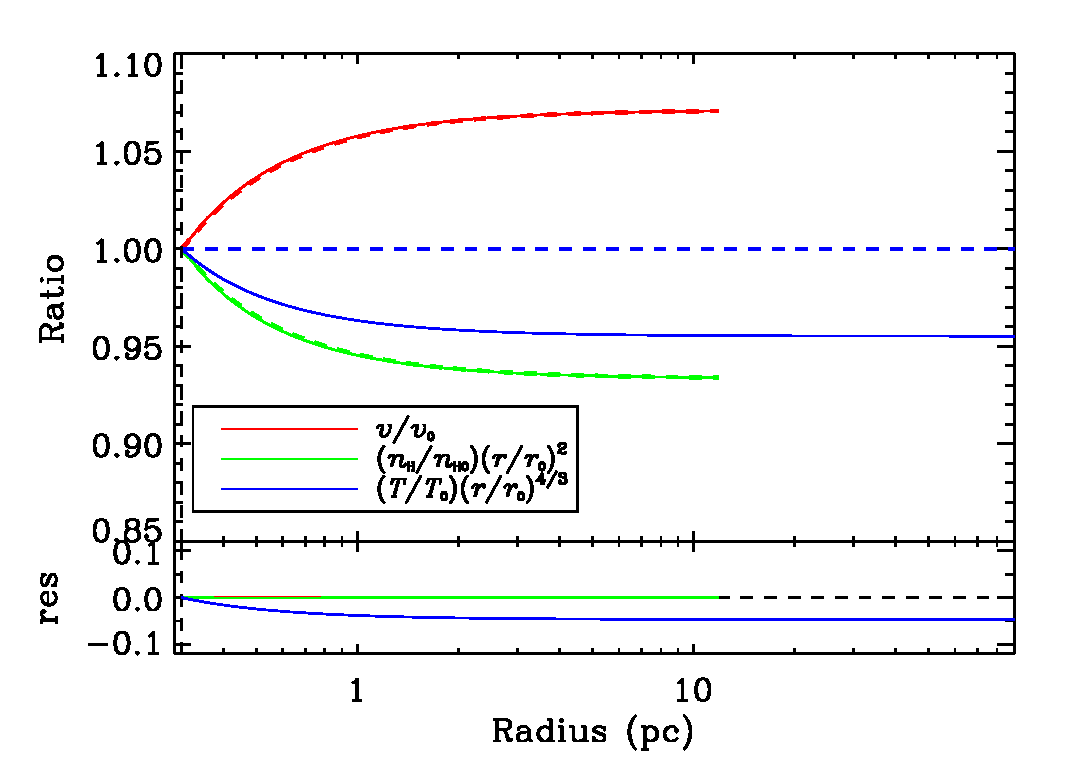
\includegraphics{figures/adia.exp_phy.eps}
  \caption{Radial profile of the flow velocity (red), density (green),
  and temperature (blue) of the adiabatic expansion. The solid lines
  follows the analytical solution in \S\ref{sec2}, and the dashed lines
  present the exponential approximations in \S\ref{sec3}. Their
  differences are plotted in the lower panel. The black
  dashed line marks the beginning radius $r_0$ of 0.3~pc.\label{fig1}}
\end{figure}

\end{document}


